\chapter{Case}



\section{Background}
The health information system in Rwanda is now going through a transition phase. 
\begin{quote}
We'd like to transition to DHIS-2 but it will require quite a bit of work on programming alerts - outgoing SMS messages - and setting up an interface for defining alert levels (ceilings) at which point the messages are sent.
\end{quote}
They are now in some way trying to transition from a series of systems to an open source software called DHIS2, see section \ref{sec:dhis}, page \pageref{sec:dhis}.
The benefits in switching to the DHIS2 is many. For starters it is an open source software. Currently parts of the health information system is contracted to companies in the private sector using proprietary software. 
Open source is free. Propietary software is not. Clearly the transition will have some finacial benefits. 
One example is a contract currently worth 300 000\$ pr. year will due to the transiton become terminated.
As one goverment employee puts it:
\begin{quote}
It is costly for the Ministry to maintain their infrastructure and is not open source.
\end{quote}
The transition from propietary software also puts the governement in control of their own software and becoming independent from companies as it relates to bug fixes, adding functionality and so forth.
The government is made up of different departments. Different departments leads to the formation of silos. Silos makes it hard to co-operate, making interoperability an issue. 
Also propietary software usually has restrictions, which contributes to the formation of silos. 
Open source software has no restrictions, which makes easy to modify and fit to the workflow and software of other departments. 
Thus making interoperability easier. 
Making the transition also leads to some added functionality, like charts for data analysis, using GIS placing data on the map, but it is also opens a door for alot of possibilites. 


\section{Current situation}
This case mainly concerns Health Management Information System and their implementation of DHIS2. HMIS is a part of the Health Ministy in Rwanda. For this paper, DHIS2 servers are run by HMIS, so a DHIS2 server is the same as an HMIS server. 
HMIS got the main responsibility to manintain and to facilitate the flow of health data in Rwanda. Even though they are the people with the main respnsibililty, as described earlier, there are other actors as well.
\begin{figure}
\centering
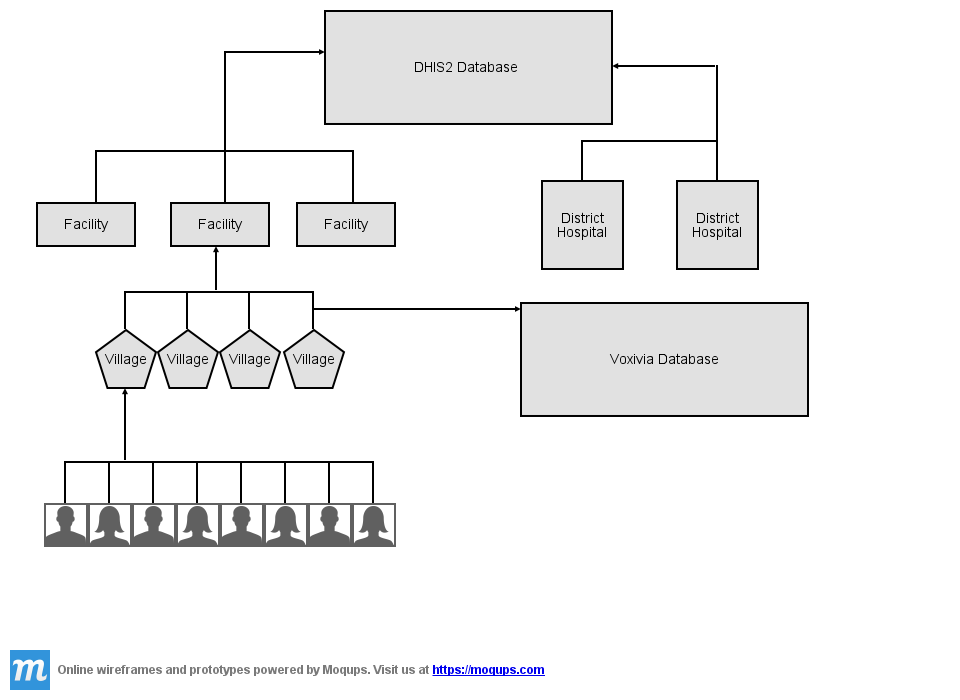
\includegraphics[width=12cm]{empirical/images/dataflow}
\label{fig:dataflow}
\caption{Dataflow}
\end{figure}
For an example there is Voxiva. A propietary software company that currently is supporting the data flow to the government using a voice response system, see figure \ref{fig:dataflow}. 
In figure \ref{dataflow} you can see how the data flows from users all the way to the DHIS2 database. If you take the route from users to the DHIS2 database, the data from users to health facilites are paper based.
The data flow that goes through the paper based system would greatly benefit from transitioning to an electronic based system.
Since DHIS2 does not support data specific to villages, another system is used to support this, currently delivered by Voxiva.
In short, making the users report data twice at the village level. One time electronicly to the Voxiva system, and one time via the paper based system to the health facility.
The paper based data collected at the health facilities are entered by data managers and then pushed to the DHIS2 databases. Data at the health facilities are aggregated by the data managers, so one cannot tell the difference between villages. 
The government would like to transision to DHIS2, but since data is aggregated at the facility level when using DHIS2, one has to use the Voxiva system for village specific data.
One typical scenario is when a village is running empty of some drug. Another village connected to the same health facility has to much of the same drug. DHIS2 would report the drug stock to be allright since the data is aggregated.
One cannot ignore this problem so HMIS is still dependent on Voxiva's system for problems like these.  
Clearly one could benefit from some interoperability. Since the data is reported twice, the system could exchange data and make life easier for the users. 

\subsection{External Systems and DHIX}
\subsubsection{DHIX}
DHIX is not an abbrevation, but a name for describing the systems at HMIS as a whole. This system include four instances of DHIS2, each running on a separate server with some scripts linking them together.
\begin{figure}
\centering
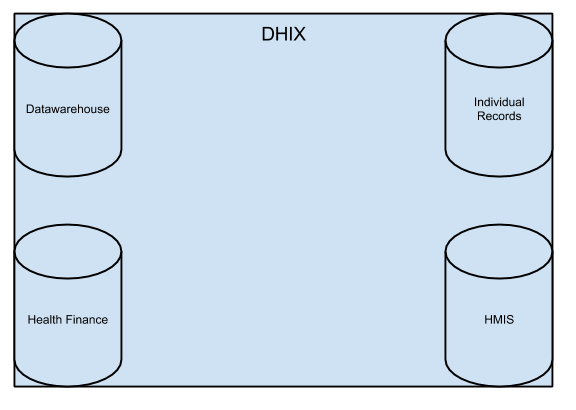
\includegraphics[width=12cm]{empirical/images/dhix_overview}
\label{fig:dhix_overview}
\caption{An overview of the DHIS2 servers at the HMIS}
\end{figure}

\begin{description}
\item[HMIS]This server contains general statistics about Rwanda's health.
\item[Health Finance]Contains information about performed health services throughout districts. This data is used for the Performance Based Financing or PBF\nomenclature{PBF}{Performance Based Financing}. 
\item[Individual Records]HMIS has a dedicated server containing information about individuals using the tracker module in DHIS2.
\item[Datawarehouse]This collects data from other DHIS2 instances. Data is pushed to this server about once a month.
\end{description}

\subsubsection{External Systems}
\begin{figure}
\centering
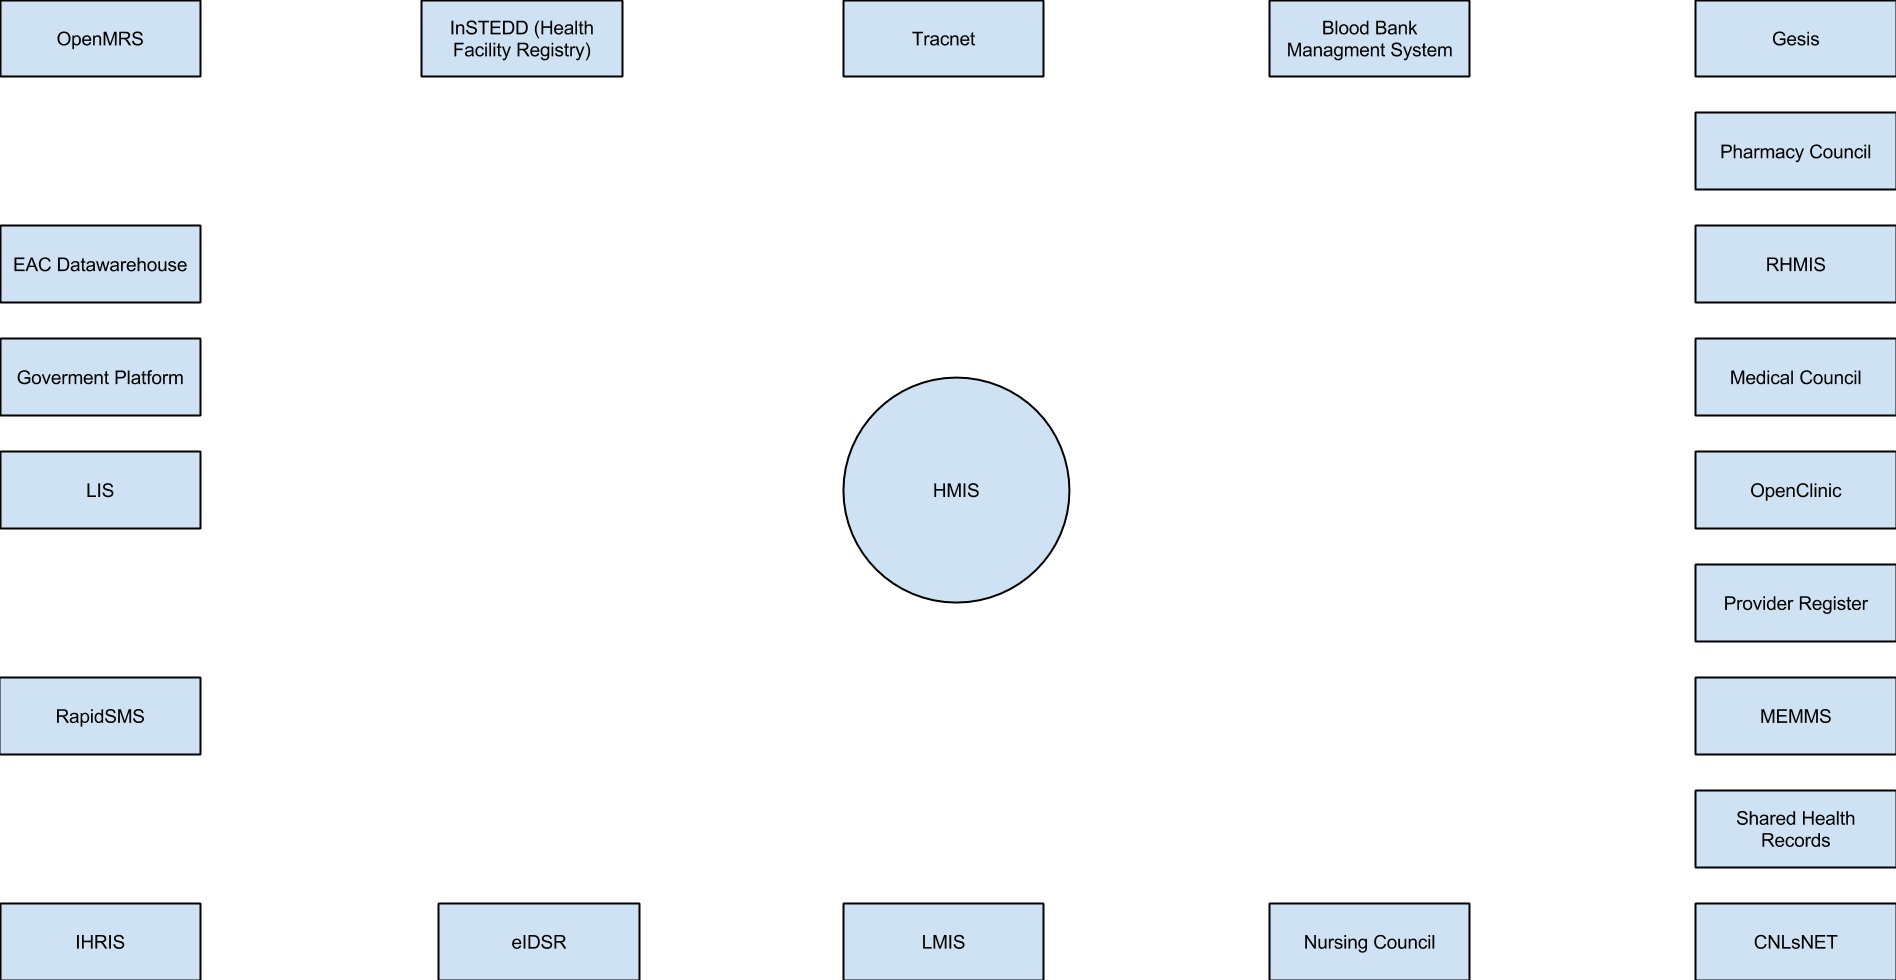
\includegraphics[width=12cm]{empirical/images/context}
\label{fig:context_systems}
\caption{Overview of systems included in the Health Information System of Rwanda}
\end{figure}
Figure \ref{fig:context_systems} shows the systems mapped during the case.
All of these systems has some relation to the DHIX and interoperabililty between the external systems and DHIX would be of benefit.
As mentioned, the Health Information system in Rwanda is going through a transition. 
Therefore, it is likely that there is some of these systems that could easaly do the switch from the old system to DHIS2 and easaly be integrated in DHIX.
This would require a huge study that I did not have the time to do during this case study, but is definitively recommended.  
I got the chance to study one of these systems in some detail and it is presented in short here. 
\subsection{Malaria Surveliance}
The purpose of this system is to map were there is an outbreak of malaria in order to initiate countermeasures.
The malaria surveliance project consists of two main branches. 
\subsubsection{Sentinel Surveliance}
The malaria sentinel project is implemented and is currently reporting weather data and malaria cases, with some extra information.
The purpose of this instance is to map all malaria cases based on their geographical location and see if there is a connection with malaria data and weather data.  
\begin{figure}
\centering
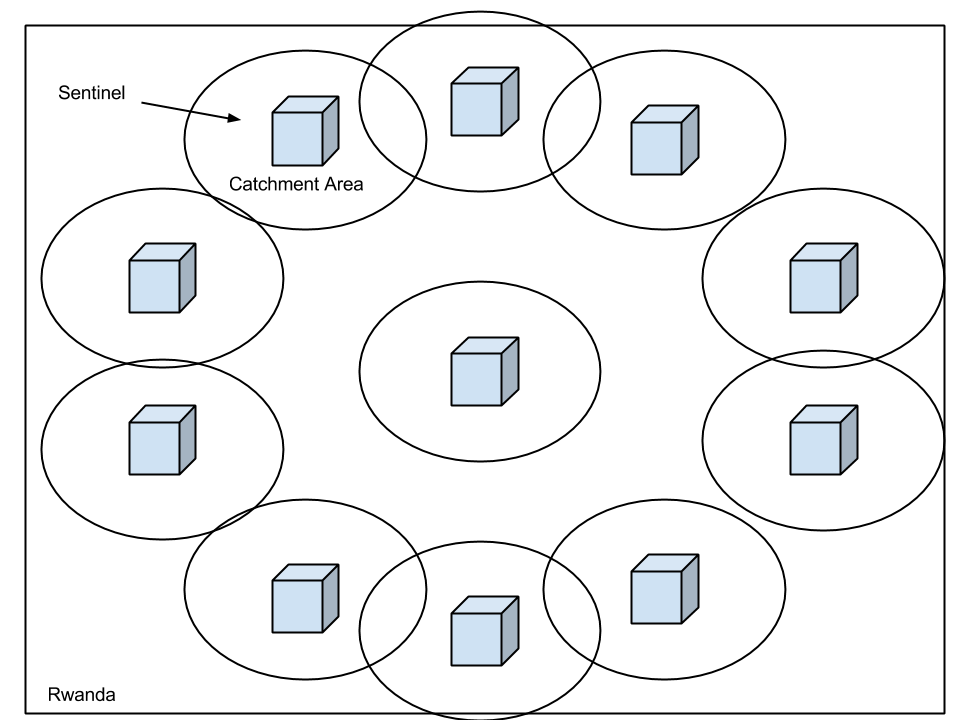
\includegraphics[width=12cm]{empirical/images/sentinel_surveliance}
\label{fig:sentinel_surveliance}
\caption{Sentinel Surveillance}
\end{figure}
The sentinels are differents stations spread throughout Rwanda, see figure \ref{fig:sentinel_surveliance}. Adding up the sentinels catchment area they should cover all of Rwanda. 
Currently these stations data flow is not integrated in DHIS2. The data being reported should happen daily. This is currently supported by DHIS2 and would be solved by making some predefined forms for the staff making the reports.
A very simple task, but it needs to be coordinated by the responsible so that everybody is onboard with the solution.
DHIS2 is currently supporting all the requirements, but in order to make the transistion the personell doing the reporting has to be trained and take part in the transition.
\subsubsection{Active Surveliance}
Active Surveliance is another branch of the malaria surveillance. The thing is, one wishes for data from the place were the malaria was first noticed.
This kind of data would include if the infected person has bednets, if others in the same house has malaria and other contextual data in hope of seing a pattern to what is most likely to make a person infected. 
Currently the health personell is using a paper based reporting form, but would like to transition to an electronic based report. See appendix \ref{chap:malaria_reporting_form} for an example of a paperbased reporting form.
The technology that the health workers currently are equipped with is usally regular simple phones that could interact with DHIS2 with SMS. 
DHIS2 is supposed to support this feature, but it is not been properly tested. 
A requirement is that one would have to set up a SMPP\nomenclature{SMPP}{Simple Message Pear-to-Pear} gateway with a local teleoperator. In this case the most likely teleoperator in Rwanda would be MTN.
The technical expertise for this kind of functionality is not the main obstacle. It's the bearucracy of decision making. 
The decicion process is long and it takes a while just to map who to talk to about what before one could even start setting up the necessary components.

As one would notice, the technology is already in place.




\section{Future goal}

\subsection{Intraoperability}
 
\subsection{Interoperability}
\begin{figure}
\centering
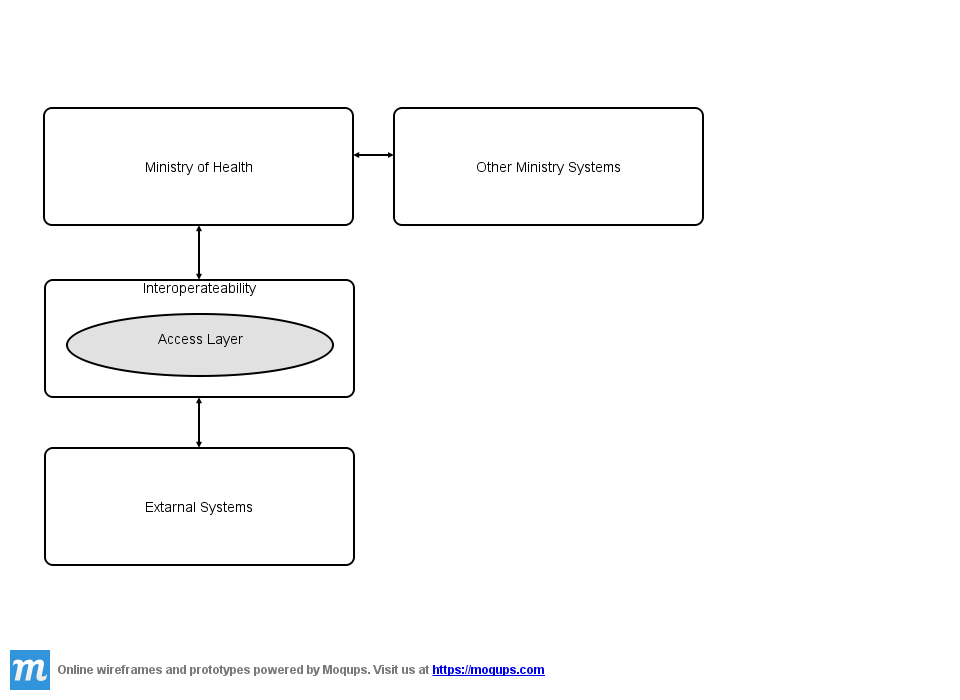
\includegraphics[width=12cm]{empirical/images/future_design_rwanda}
\label{future_design}
\caption{Future Design}
\end{figure}
\subsubsection{Health Facility Registry}
The HMIS has a vision on how they would like to interact with other systems, see \ref{future_design}. HMIS would like to collect all Ministry of Health systems under one roof. Then they would like to make some kind of interface between health ministry and other ministry systems. The specifics of how this is going to work are not decided yet. The ministry of health would like to be able to exchange data with external systems as well. This is done via an access layer. Between this access layer one would be able to synchronize data with external systems. For instance, there is a system called Voxivia that has data that is more specific than what is currently supported by the DHIS2. These data would be of great benefit to the HMIS. 




\section{Challenges}



\section{My role and case results}
\subsection{4 projects}
\subsection{The Landing}
\subsubsection{Result}
\subsection{Future Project}